\section{Preprocesado de los datos}

Nuestro conjunto de datos se compone de tres ficheros:

\begin{enumerate}
	\item \texttt{lateralidad0.arff} : 439 muestras de la lateralidad izquierda del pubis.
	\item \texttt{lateralidad1.arff} : 453 muestras de la lateralidad derecha del pubis.
	\item \texttt{completo.arff} : 892 muestas de ambas lateralidades, se compone de los dos ficheros antes en conjunto.
\end{enumerate}

\begin{figure}[H]
	\begin{lstlisting}[language={}]
	NoGrooves,Absence,Defined,Absent,Defined,Present,Absent,Absent,FormedWithoutRarefactions,36
	\end{lstlisting}
	\caption{Ejemplo de un dato cuya edad de muerte es 36 años, del conjunto de datos \texttt{completo.arff}.}
	\label{fig:ejemplo_dato}
\end{figure}

Como vemos en la figura \ref{fig:ejemplo_dato} los datos tienen asignados valores categóricos para cada característica, y finalmente la edad a la que murió la persona con las características asociadas.

\subsection{Transformación de las características}

De cara a poder trabajar con estos datos para aplicar el sobremuestreo a los datos y después regresión simbólica tenemos que transformar estos valores categóricos a valores numéricos.

Para esto simplemente leeremos los valores y a cada característica le asignaremos un valor entre uno y el máximo número de posibles valores para dicha característica, de forma que una característica con dos posibles valores será $1$ o $2$, dependiendo de cual de los dos valores aparezca.


\begin{table}[H]
\centering
\resizebox{\textwidth}{!}{%
\begin{tabular}{|c|c|c|c|}
\hline
                                                      & \textbf{Variable asignada} & \textbf{Valor categórico}       & \textbf{Valor numérico asignado} \\ \hline
\multirow{6}{*}{\textbf{Crestas y surcos}}            & \multirow{6}{*}{$x_0$}     & No hay surcos                   & 1                                \\ \cline{3-4}
                                                      &                            & Restos de surcos                & 2                                \\ \cline{3-4}
                                                      &                            & Surcos poco profundas           & 3                                \\ \cline{3-4}
                                                      &                            & Crestas en formación            & 4                                \\ \cline{3-4}
                                                      &                            & Crestas poco profundas          & 5                                \\ \cline{3-4}
                                                      &                            & Crestas con porosidad regular   & 6                                \\ \hline
\multirow{3}{*}{\textbf{Superficie porosa irregular}} & \multirow{3}{*}{$x_1$}     & No                              & 1                                \\ \cline{3-4}
                                                      &                            & Medianamente                    & 2                                \\ \cline{3-4}
                                                      &                            & Si                              & 3                                \\ \hline
\multirow{2}{*}{\textbf{Borde superior}}              & \multirow{2}{*}{$x_2$}     & No definido                     & 1                                \\ \cline{3-4}
                                                      &                            & Definido                        & 2                                \\ \hline
\multirow{2}{*}{\textbf{Nódulo óseo}}                 & \multirow{2}{*}{$x_3$}     & Ausente                         & 1                                \\ \cline{3-4}
                                                      &                            & Presente                        & 2                                \\ \hline
\multirow{2}{*}{\textbf{Borde inferior}}              & \multirow{2}{*}{$x_4$}     & No definido                     & 1                                \\ \cline{3-4}
                                                      &                            & Definido                        & 2                                \\ \hline
\multirow{2}{*}{\textbf{Borde dorsal}}                & \multirow{2}{*}{$x_5$}     & No definido                     & 1                                \\ \cline{3-4}
                                                      &                            & Definido                        & 2                                \\ \hline
\multirow{2}{*}{\textbf{Plataforma dorsal}}           & \multirow{2}{*}{$x_6$}     & Ausente                         & 1                                \\ \cline{3-4}
                                                      &                            & Presente                        & 2                                \\ \hline
\multirow{3}{*}{\textbf{Bisel ventral}}               & \multirow{3}{*}{$x_7$}     & Ausente                         & 1                                \\ \cline{3-4}
                                                      &                            & En proceso de formación         & 2                                \\ \cline{3-4}
                                                      &                            & Formado                         & 3                                \\ \hline
\multirow{5}{*}{\textbf{Borde ventral}}               & \multirow{5}{*}{$x_8$}     & Ausente                         & 1                                \\ \cline{3-4}
                                                      &                            & Parcialmente formado            & 2                                \\ \cline{3-4}
                                                      &                            & Formado sin excrecencias        & 3                                \\ \cline{3-4}
                                                      &                            & Formado con pocas excrecencias  & 4                                \\ \cline{3-4}
                                                      &                            & Formado con muchas excrecencias & 5                                \\ \hline
\end{tabular}%
}
\caption{Transformaciones aplicadas a las características antes de realizar el sobremuestreo.}\label{table:transformaciones_numericas}

\end{table}

Con respecto a las etiquetas, aunque en un principio este problema esté pensado para clasificación y se divida en diez fases, contamos con el conjunto de datos preparado para regresión, es decir, con un valor numérico asignado.

% TODO : A ver que hago con esta parte de Borderline-SMOTE, en principio la voy a dejar por si me sirve para la segunda parte de clasificación

\subsection{Algoritmo Borderline-SMOTE}

El algoritmo Borderline-SMOTE \cite{BL-SMOTE} se basa en una variante de SMOTE \cite{SMOTE}.

SMOTE se trata de un método para conseguir nuevos datos de las clases minoritarias de forma sintética.

Las clases minoritarias se sobremuestrean tomando cada muestra de dicha clase minoritaria, e introduciendo valores sintéticos a los largo del segmento que une a todos o a cualquiera de los $k$ vecinos más cercanos de la clase. Dependiendo de la cantidad de datos sintéticos a generar se escogerá el valor de $k$ para seleccionar más o menos vecinos.


\begin{figure}[H]
	\centering
	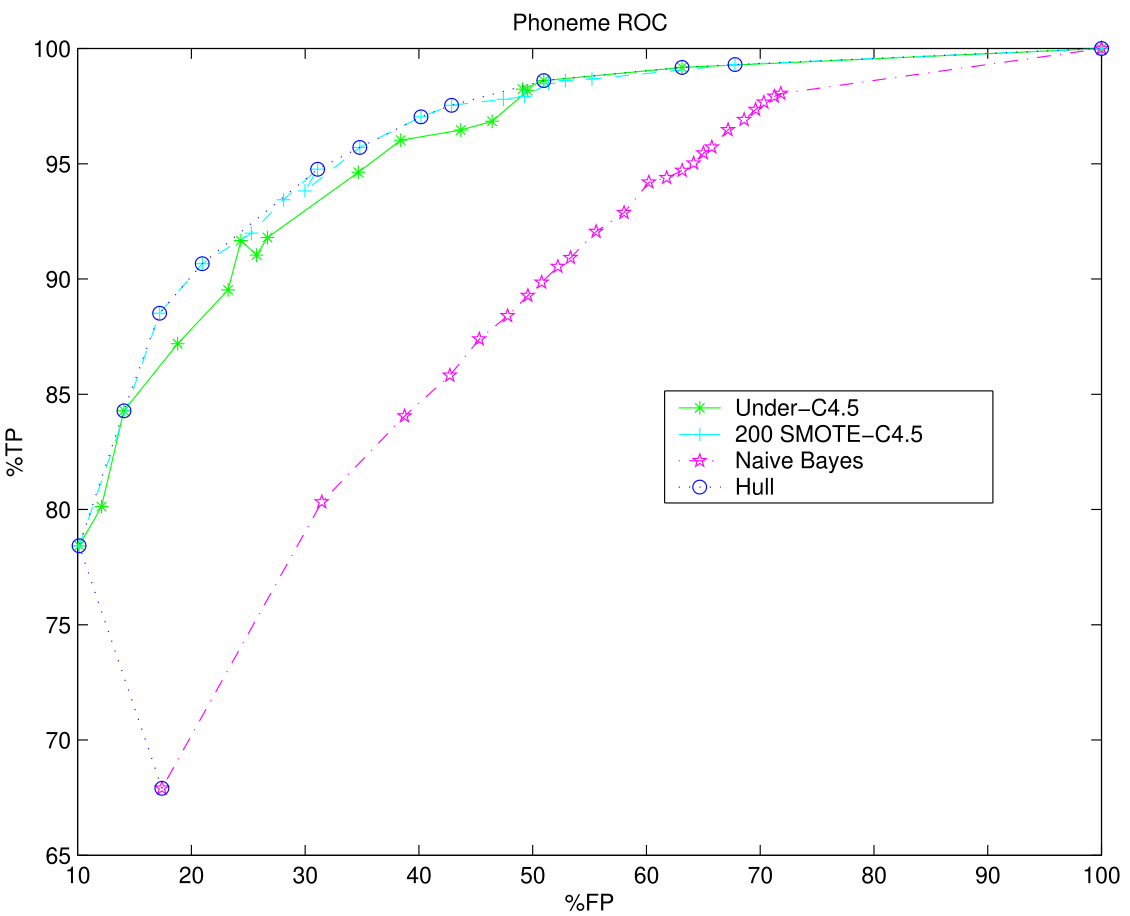
\includegraphics[scale = 1]{ej_smote.png}
	\caption{Comparación de SMOTE con otros métodos de sobremuestreo en el conjunto de datos Phonome. En el eje X los falsos positivos y en el eje Y los verdaderos positivos. Imagen obtenida de \cite{SMOTE}.}
	\label{fig:comparacionSMOTE}
\end{figure}

Como vemos en la figura \ref{fig:comparacionSMOTE}, este método se comporta bastante bien en comparación con otros métodos y es capaz de obtener buenos resultados, sin embargo, tiene algunos problemas.

Uno de estos problemas es que cuando existe ruido entre las clases, o las clases se encuentran dispersas por el espacio de valores, gran parte de los valores sintéticos se encontrarán en una zona del espacio que no corresponde a su clase.

Este problema se hace mucho más presente en nuestro caso, al contar con tantas clases y con tantas características, y para resolverlo utilizaremos la variante Borderline-SMOTE.

Esta variante, basada en SMOTE, propone buscar los límites en el espacio de valores de la clase a obtener nuevos datos sintéticos, de forma que cuando se generen dichos datos nuevos, estén dentro de dichos límites. De esta forma evitamos problemas con conjuntos de datos con mucho ruido y múltiples clases.

En su artículo proponen dos variantes, una donde las nuevas muestras sintéticas son creadas a partir de todo el conjunto de datos, y otra donde las nuevas muestras solo se generan a partir de los datos considerados en el límite.


\begin{figure}[H]
    \centering
    \begin{subfigure}[b]{0.33\textwidth}
		  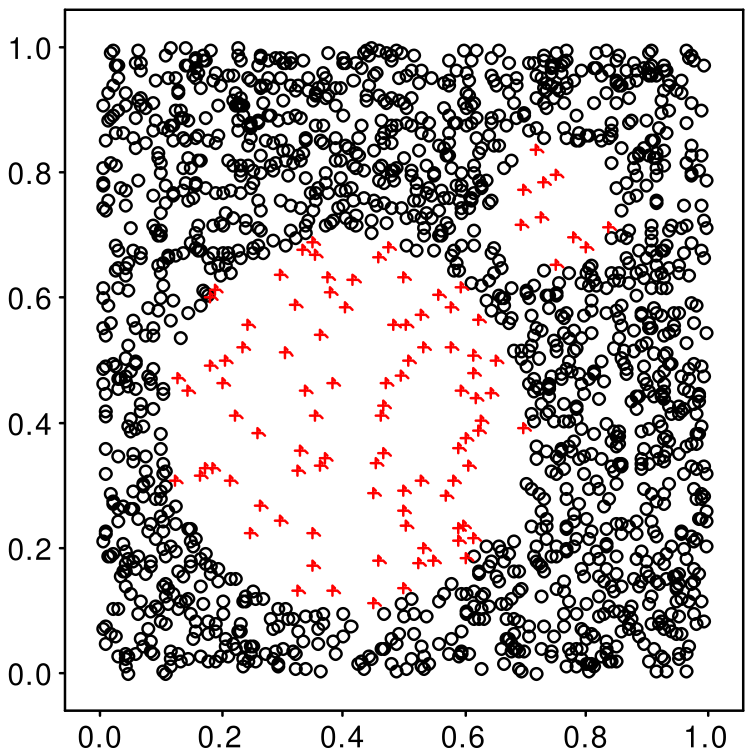
\includegraphics[width=\textwidth]{bl-smote-original.png}
        \caption{}
        \label{fig:blSMOTE-orig}
    \end{subfigure}
    \begin{subfigure}[b]{0.33\textwidth}
        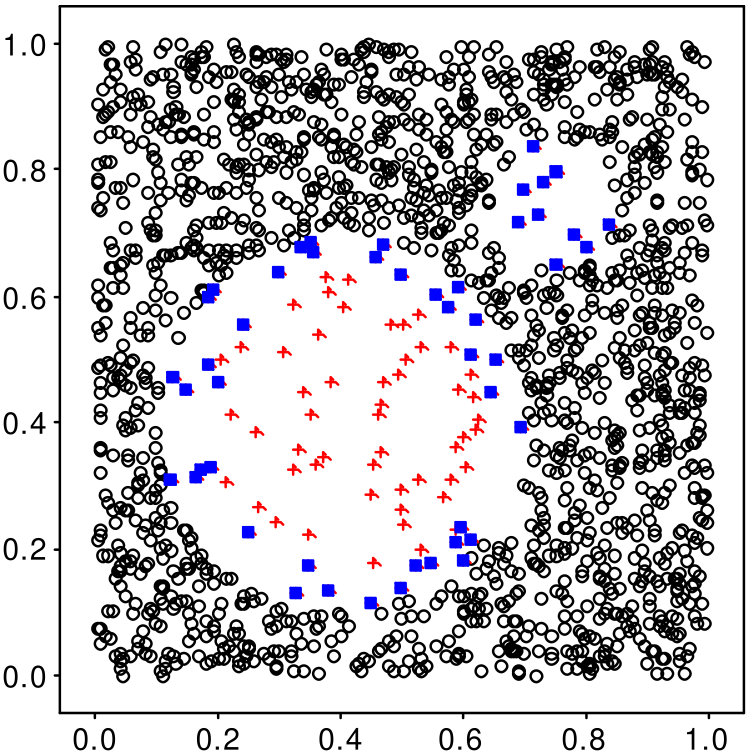
\includegraphics[width=\textwidth]{bl-smote-datos-borderline.png}
        \caption{}
        \label{fig:blSMOTE-border}
    \end{subfigure}
    \begin{subfigure}[b]{0.33\textwidth}
        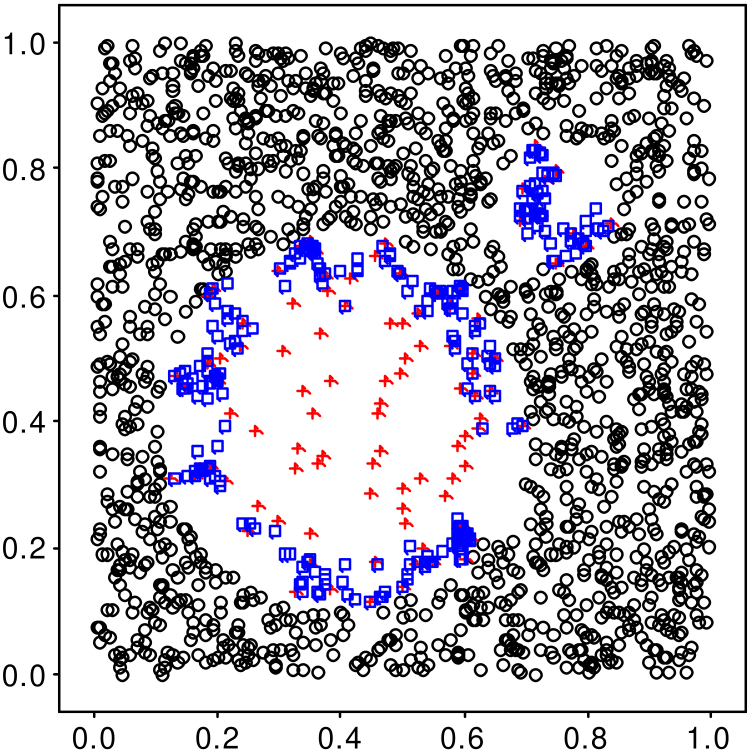
\includegraphics[width=\textwidth]{bl-smote-datos-sinteticos.png}
        \caption{}
        \label{fig:blSMOTE-sintetico}
    \end{subfigure}

    \caption{\ref{fig:blSMOTE-orig} Conjunto de datos original. \ref{fig:blSMOTE-border} datos que conforman el límite de la clase minoritaria (cuadros azules rellenos). \ref{fig:blSMOTE-sintetico} Nuevos datos generados de forma sintética dentro de los límites de la clase (cuadros azules no rellenos). Imagen obtenida de \cite{BL-SMOTE}.}
	 \label{fig:ejemploBL-SMOTE}

\end{figure}


\begin{figure}[H]
    \centering
	 \begin{subfigure}[b]{\textwidth}
		 \centering
		 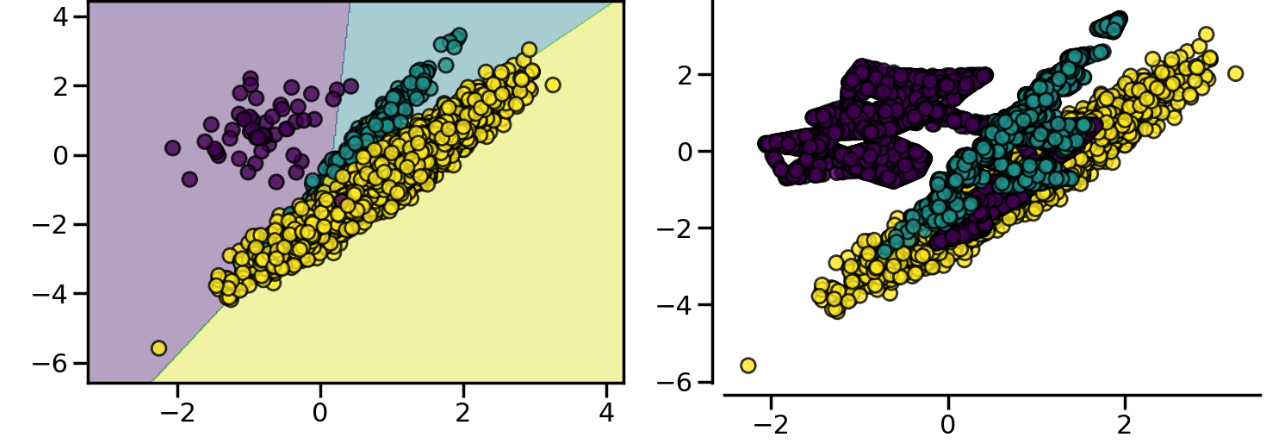
\includegraphics[width=0.8\textwidth]{resampling_smote.png}
		 \caption{A la izquierda bordes de las clases, y a la derecha sobremuestreo con SMOTE}
		 \label{fig:SMOTE-cmp}
	 \end{subfigure}

    \begin{subfigure}[b]{\textwidth}
		 \centering
		  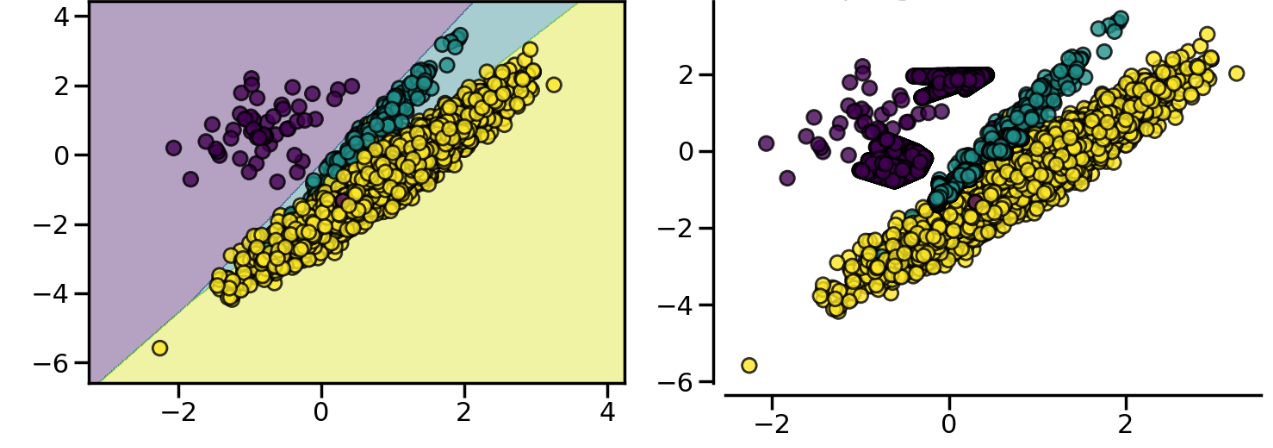
\includegraphics[width=0.8\textwidth]{resampling_blsmote.png}
        \caption{A la izquierda bordes de las clases, y a la derecha sobremuestreo con BorderlineSMOTE}
        \label{fig:BLSMOTE-cmp}
    \end{subfigure}

    \caption{Comparación de SMOTE y BorderlineSMOTE para un conjunto de datos generado aleatoriamente.}\label{fig:BLSMOTE-SMOTE}

\end{figure}

Esta claro que, como vemos en la figura \ref{fig:ejemploBL-SMOTE} y la figura \ref{fig:BLSMOTE-SMOTE}, esta técnica es mucho más versátil y conveniente que SMOTE, motivo por el que la utilizaremos.


De cara a su implementación se utilizará el módulo de Python \texttt{imbalanced-learn} que implementa el algoritmo de BorderlineSMOTE \cite{imblearnBLSMOTE}.



\newpage

\subsection{Resultado tras el preprocesado}

Tras aplicar todas las fases del preprocesado obtenemos los conjuntos de datos finales que utilizaremos.

\begin{figure}[H]
    \centering
	  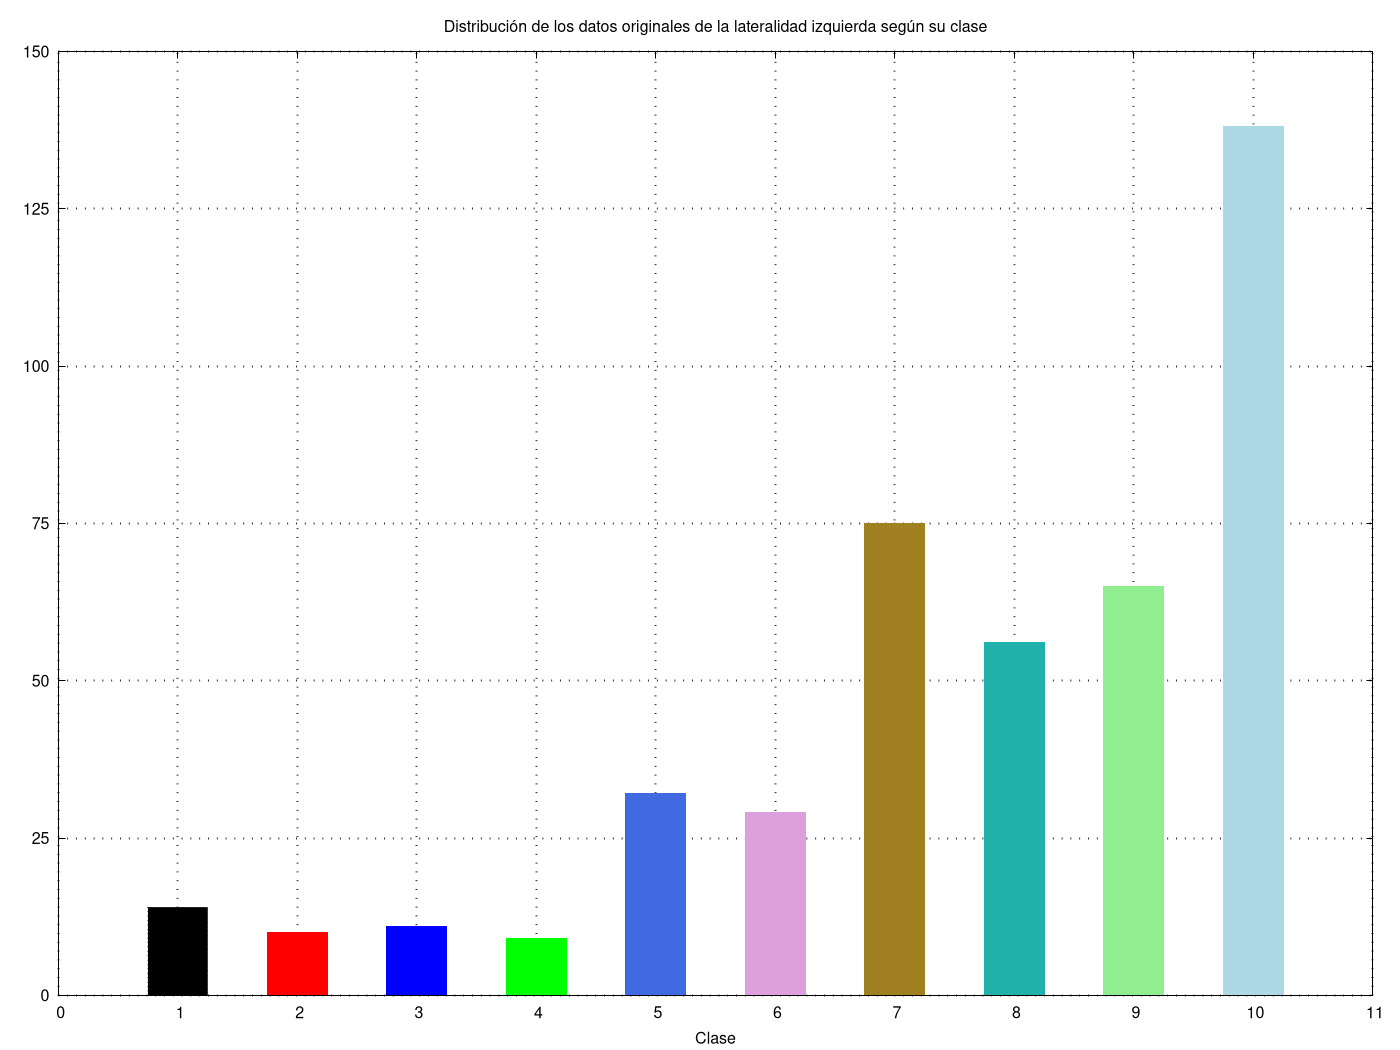
\includegraphics[width=0.6\textwidth]{conjunto_datos/num_elementos_fase_l0.png}
    \caption{Conteo de elementos por fase en el conjunto de datos original de la lateralidad izquierda.}
	 \label{fig:l0-orig}
\end{figure}

\begin{figure}[H]
    \centering
     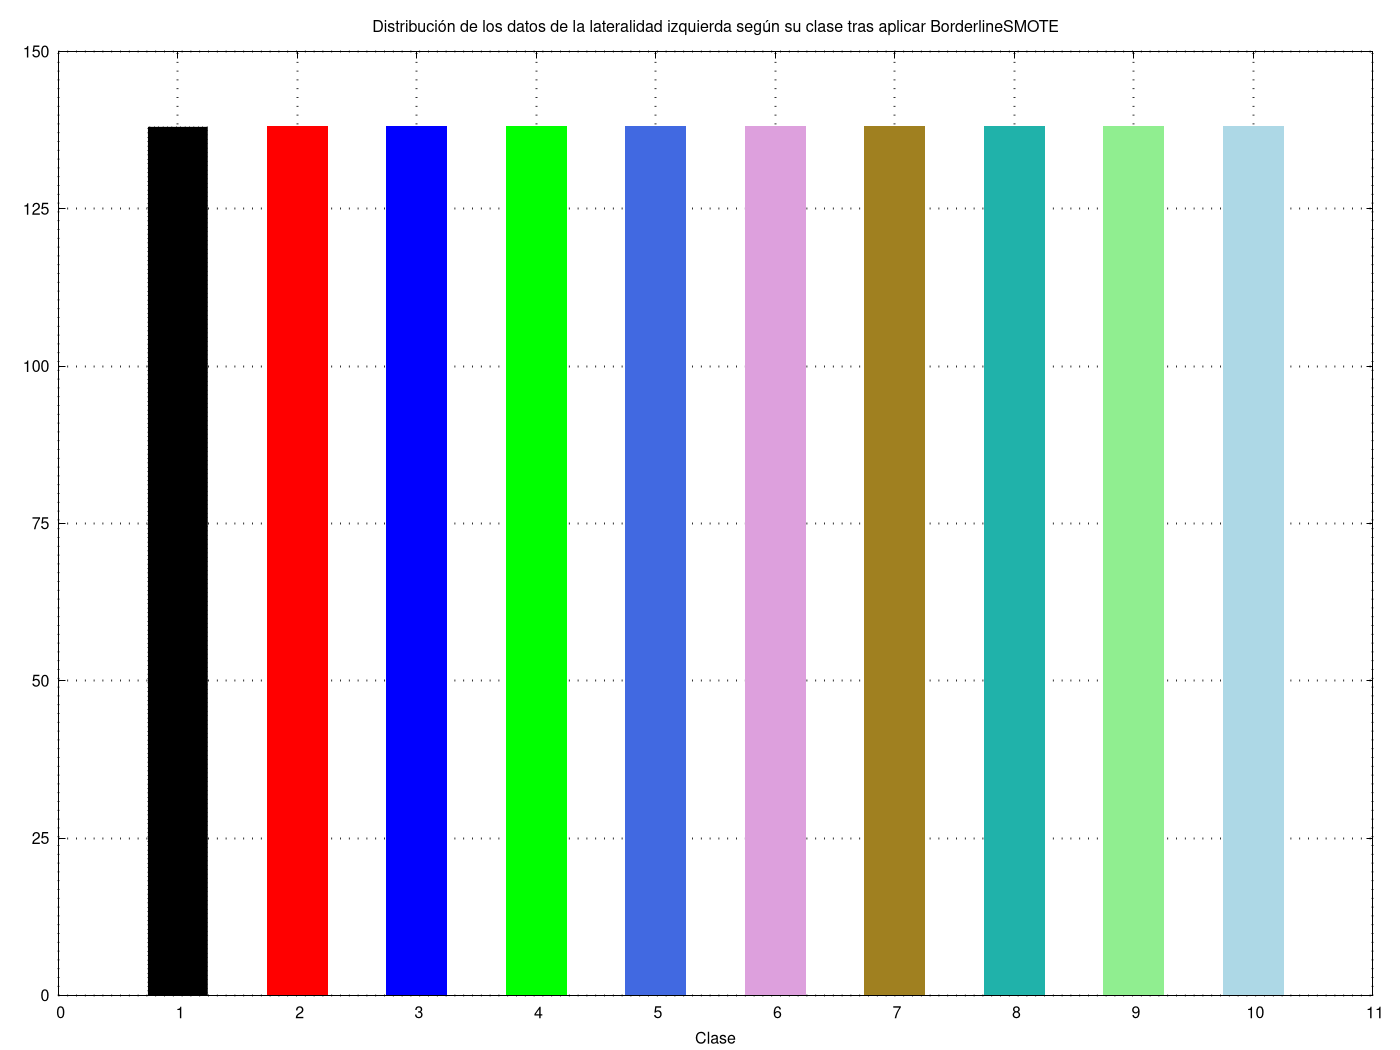
\includegraphics[width=0.6\textwidth]{conjunto_datos/num_elementos_fase_l0_BL-SMOTE.png}
    \caption{Conteo de elementos por fase en el conjunto de datos de la lateralidad izquierda tras aplicar BorderlineSMOTE.}
	 \label{fig:l0-over}
\end{figure}

\begin{figure}[H]
    \centering
	  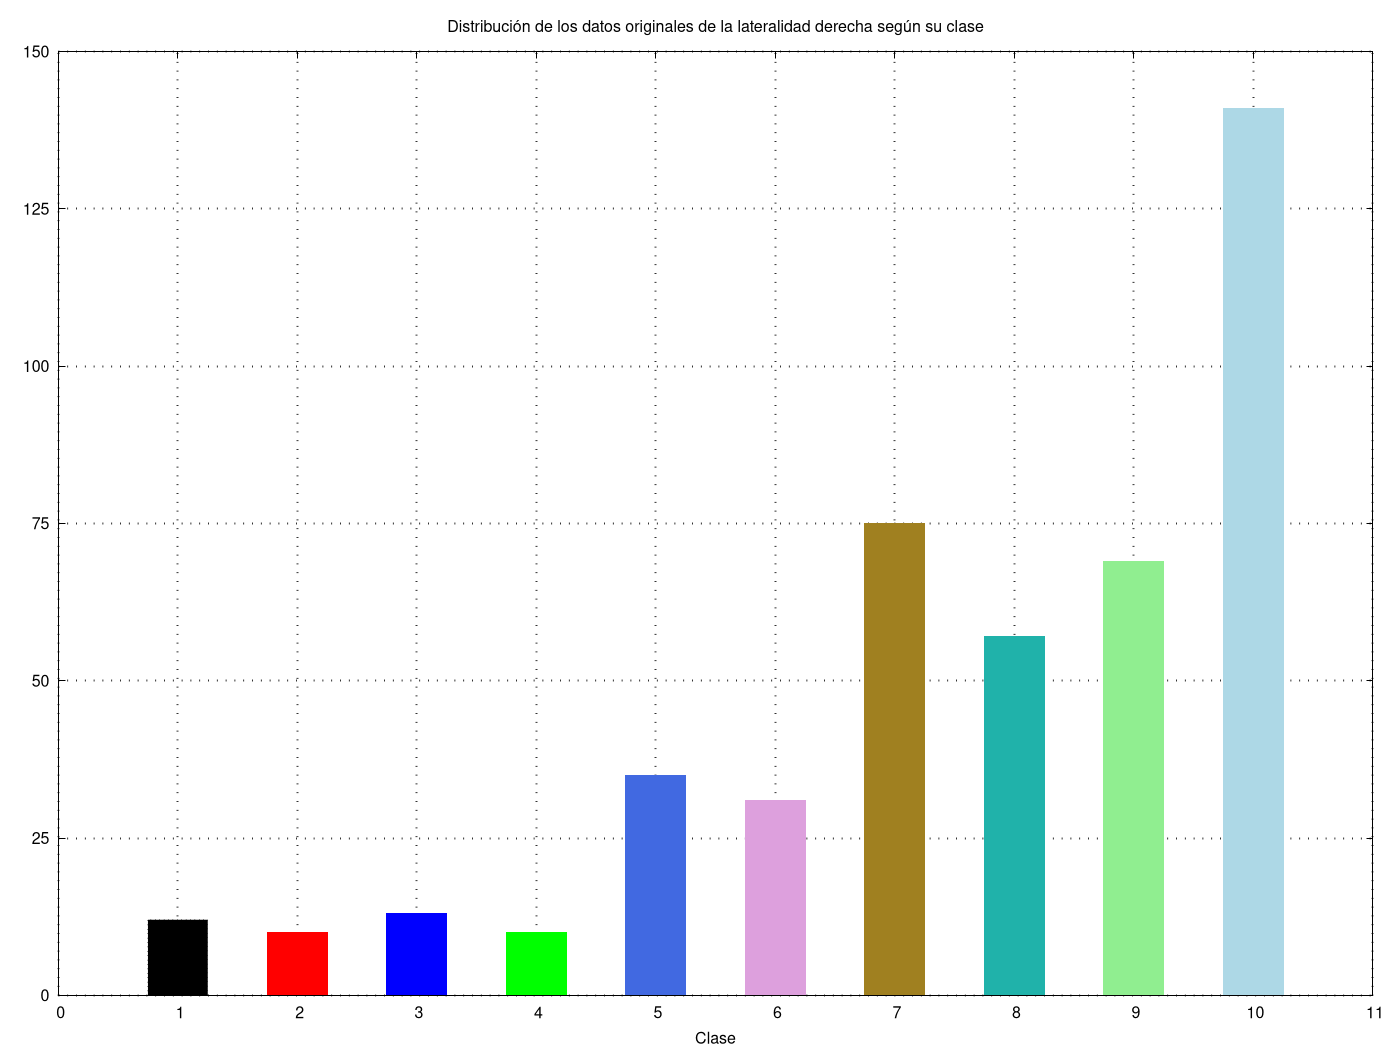
\includegraphics[width=0.6\textwidth]{conjunto_datos/num_elementos_fase_l1.png}
    \caption{Conteo de elementos por fase en el conjunto de datos original de la lateralidad derecha.}
	 \label{fig:l1-orig}
\end{figure}

\begin{figure}[H]
    \centering
     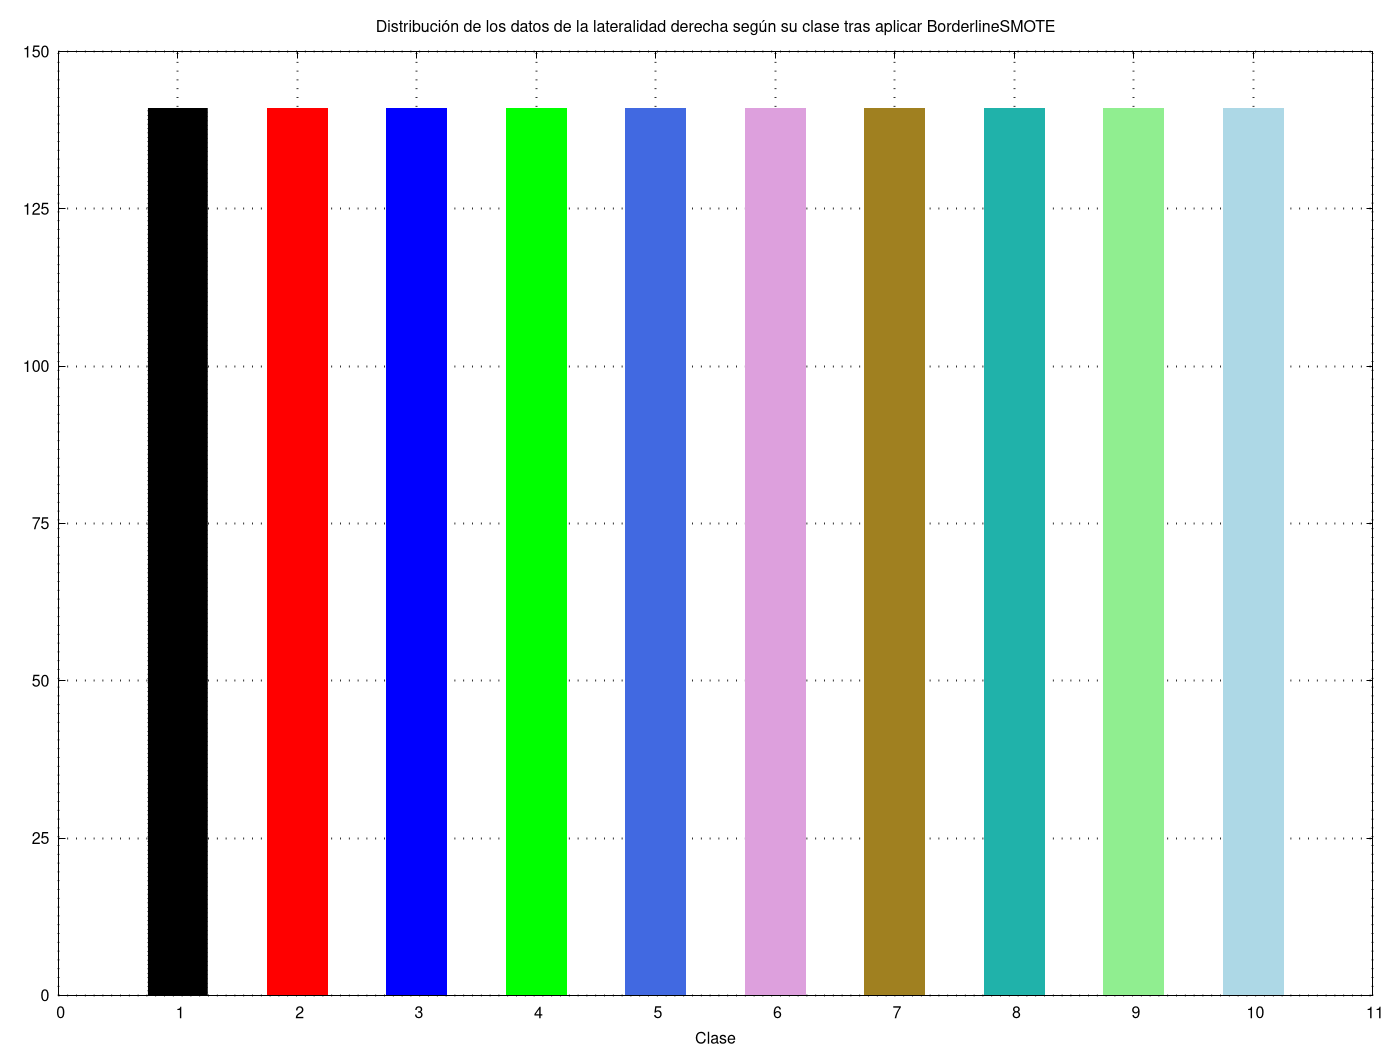
\includegraphics[width=0.6\textwidth]{conjunto_datos/num_elementos_fase_l1_BL-SMOTE.png}
    \caption{Conteo de elementos por fase en el conjunto de datos de la lateralidad derecha tras aplicar BorderlineSMOTE.}
	 \label{fig:l1-over}
\end{figure}



\begin{figure}[H]
    \centering
	  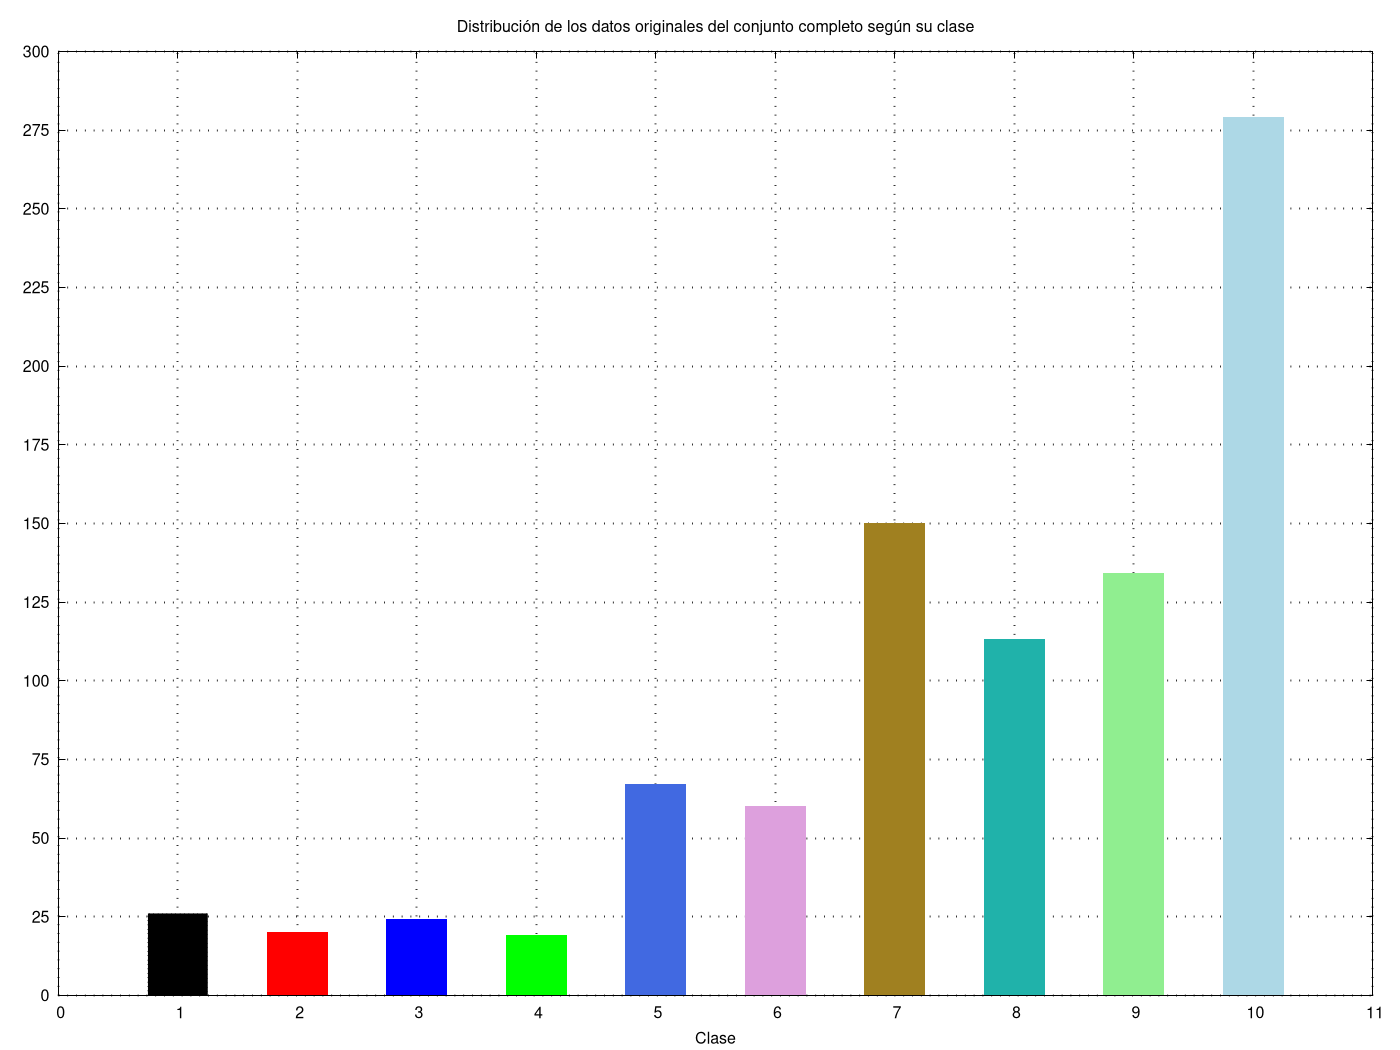
\includegraphics[width=0.6\textwidth]{conjunto_datos/num_elementos_fase_completo.png}
     \label{fig:completo-orig}
    \caption{Conteo de elementos por fase en el conjunto de datos completo original.}

\end{figure}

\begin{figure}[H]
    \centering
     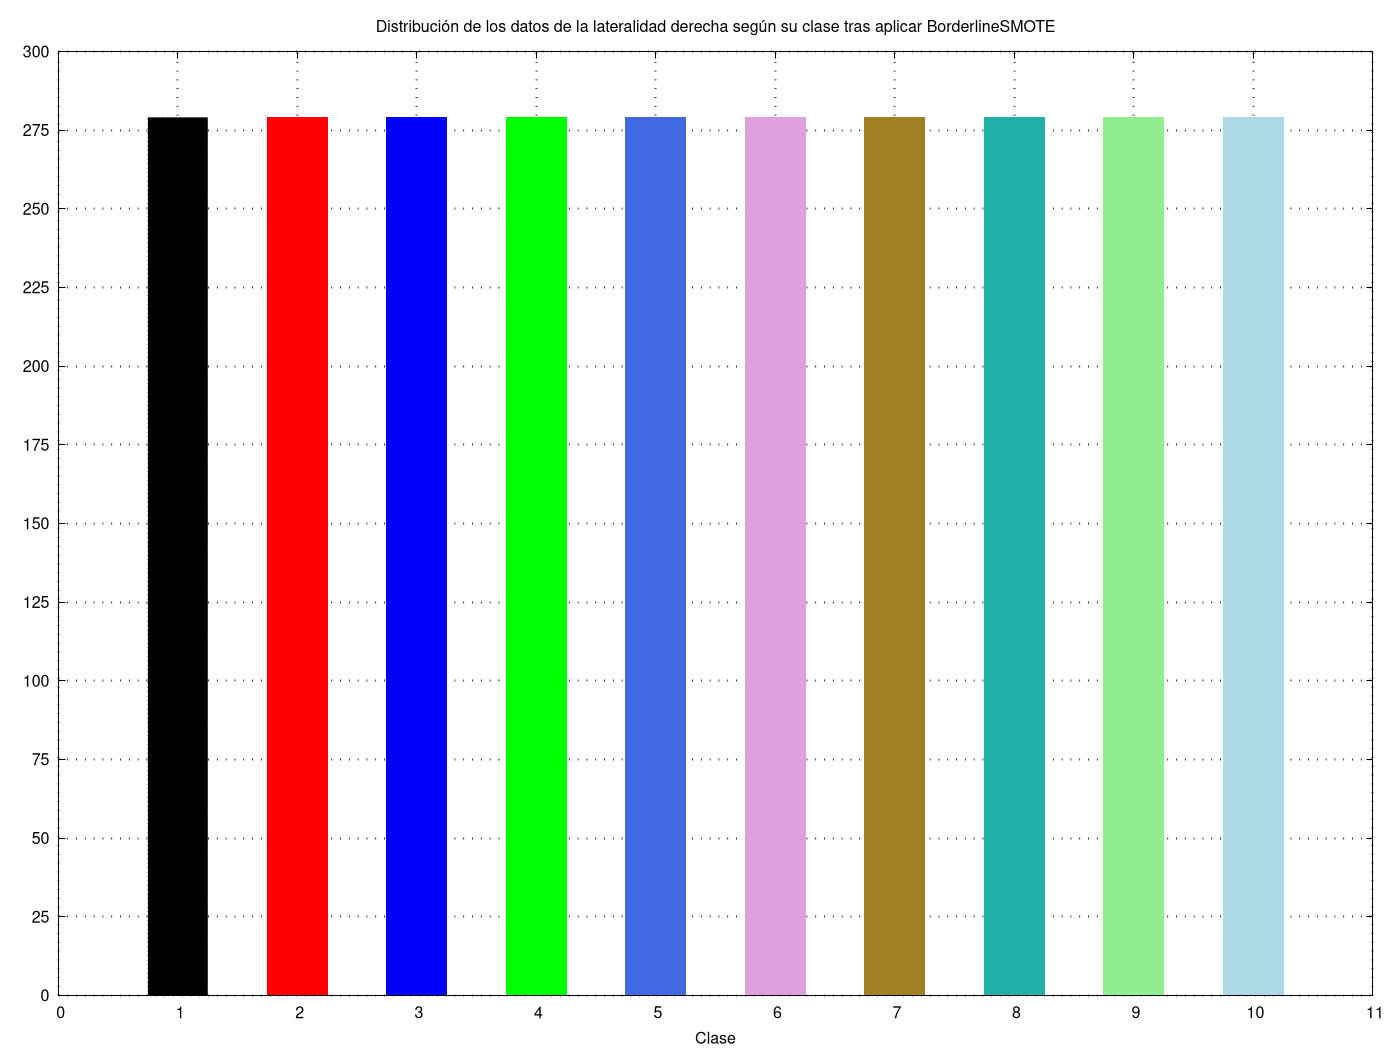
\includegraphics[width=0.6\textwidth]{conjunto_datos/num_elementos_fase_completo_BL-SMOTE.png}
    \caption{Conteo de elementos por fase en el conjunto de datos completo tras aplicar BorderlineSMOTE.}
	 \label{fig:completo-over}
\end{figure}


Como vemos en las figuras \ref{fig:l0-over}, \ref{fig:l1-over} y \ref{fig:completo-over} ya tenemos conjuntos de datos balanceado y, aplicando la propuesta de Gilbert, con una única variable que serán los conjuntos de datos que utilizaremos.
